\documentclass{article}
\usepackage{graphicx}
\usepackage{siunitx}
\graphicspath{ {images/} }
\title{Sign Problem}
\author{Grant Curell}
\begin{document}
\maketitle{}
\section{Problem}
Here, the mass m isn’t moving, and you’re applying a force F to hold it stationary. Here’s the question: What force is the pulley’s support exerting, and in which direction, to keep the pulley where it is?

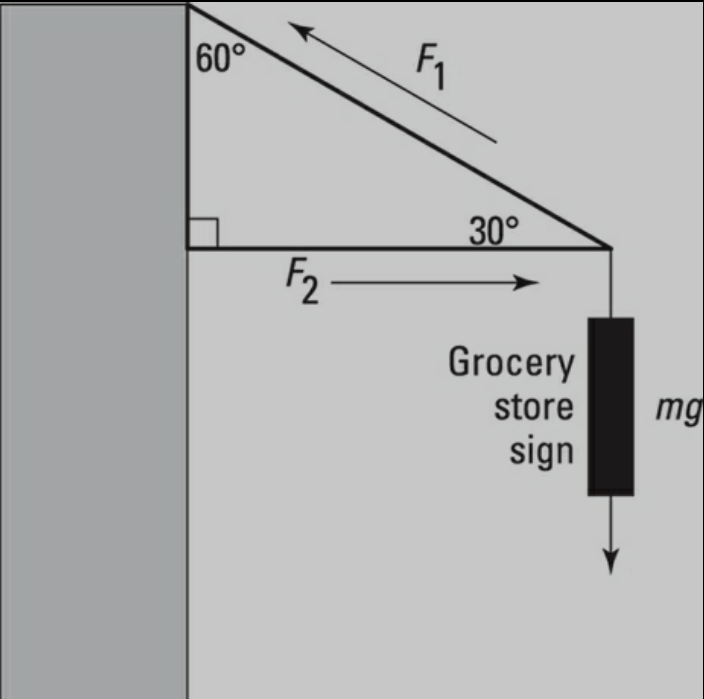
\includegraphics[width=\columnwidth]{image}
\\\\
Holzner, Steven. Physics I For Dummies (For Dummies (Math \& Science)) (p. 94). Wiley. Kindle Edition.
\\\\
\section{Solution}
\[ F_1=15N \]
\[ F_s=8N \]
\[ a=0 \]
\[ F_{sign-y}=15\cos(60) \]
\[ F_{sign-y}=7.5 \]
El letro require 8N de fuerza para sostenerse. El alambre solo puede apoyar 7.5N de fuerza en la eje y lo que es insuficiente.
\\\\
The sign requires 8N of force to support itself. The wire can only support 7.5N in the y axis, which is insufficient for the 8N required by the wire.
\section{Question}
The book used the following explanation. Mine seems logical, but is it mathematically correct?
\\\\
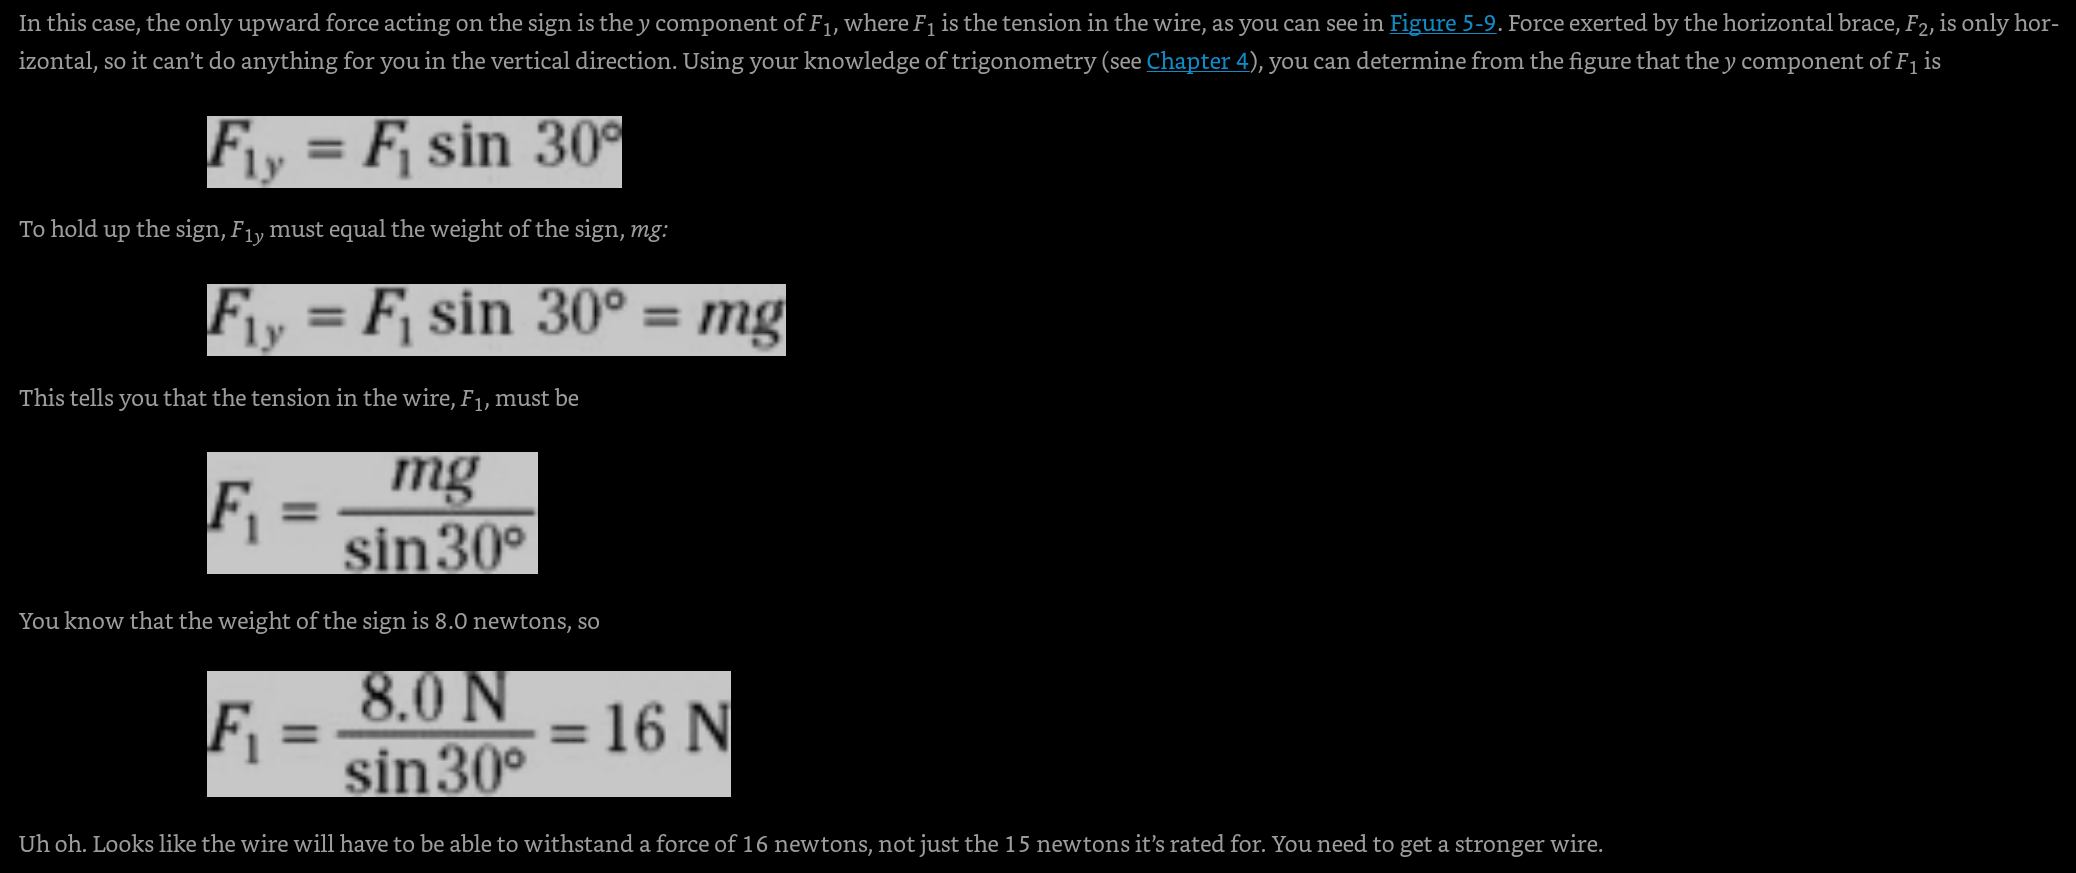
\includegraphics[width=\columnwidth]{image2}
\end{document}
